\documentclass[main.tex]{subfiles}
\begin{document}
\section{Introduction : positionnement du problème}

On va s'intéresser aux signaux analogiques vus comme des fonctions réelles

\[x : t \in \R \rightarrow x(t) \in \R\]

Les processus évoluent continûment dans le temps.\\

\begin{figure}[h!]
\centering
\begin{tikzpicture}
\sbEntree{E}
\sbComp{comp}{E}
\sbRelier[$c(t)$]{E}{comp}
\sbBloc{reg}{Structure de commande}{comp}
\sbRelier[$\epsilon$]{comp}{reg}
\sbBloc{sys}{Système}{reg}
\sbRelier[u(t)]{reg}{sys}
\sbSortie{S}{sys}
\sbRelier[$y(t)$]{sys}{S}
\sbRenvoi{sys-S}{comp}{}
\end{tikzpicture}
\caption{Asservissement analogique}
\end{figure}


La loi de commande est alors :
\begin{align*}
U(p) & = C(p).[R(p) - Y(p)], \text{ transformée de Laplace de }\\
u(t) & = c(t)*[r(t) - y(t)]
\end{align*}

\paragraph*{Problématique}
Il faut alors évaluer u(t) et le mettre en œuvre de manière analogique et/ou bon moment. Pour cela, il est nécessaire de calculer en temps réels et d'adapter u(t).\\

La solution est d'exploiter un calculateur numérique couplé à de l'électronique numérique pour implémenter la loi de commande.
Par exemple :
\begin{itemize}
\item ordinateur à base de microprocesseurs cadencés par une horloge interne
\item micro-contrôleurs
\item DSP (Digital Signal Processing, puce à usage spécifique, non modifiable)
\item Arduino
\end{itemize}

L'information est transmise par des signaux binaires eux-mêmes étant des signaux numériques. Cette information ne transporte pas l'énergie nécessaire pour contrôler le processus, mais seulement la loi de commande.

Les signaux numériques évoluent de manière discrète à des instants régulièrement espacés par un intervalle de temps donné par la période de l'horloge $T_h = \frac{1}{f_h}$.

On pose l'hypothèse que $T_h$ est constante donc les différents instants correspondent à $k.T_h$ où $k\in\mathbb{N}$.\\

\subsection*{Définition}
Le signal numérique $u_k$ est défini comme une suite numérique :
\begin{align*}
\mathbb{N} & \rightarrow \mathbb{R} \\
k & \mapsto U_k
\end{align*}

\subsection*{Calculateurs numériques}
Ils servent à implémenter les lois de commande, c'est-à-dire les règles mathématiques d'évolution des signaux.

\begin{figure}[h!]
\centering
\begin{tikzpicture}
\sbEntree{E}

\sbBloc{calc}{Calculateur numérique}{E}
\sbRelier[$e_k$]{E}{calc}

\sbBloc{cna}{CNA}{calc}
\sbRelier[$u_k$]{calc}{cna}

\sbBloc{sys}{Système analogique}{cna}
\sbRelier[$u(t)$]{cna}{sys}

\sbSortie{S}{sys}
\sbRelier[$y(t)$]{sys}{S}

\sbDecaleNoeudy[4]{S}{R}
\sbBlocr[12]{can}{CAN}{R}
\sbRelieryx{sys-S}{can}
\sbRelierxy{can}{calc}

\end{tikzpicture}
\caption{Interfaçage Numérique / Analogique}
\end{figure}

\noindent Remarque :\\
CAN : Convertisseur Analogique Numérique\\CNA : Convertisseur Numérique Analogique\\

L'horloge permet le fonctionnement synchrone des différents composants de la structure de l'asservissement numérique.

\section{Modélisation des signaux échantillonnés}
\subsection*{Échantillonnage}
\begin{defin}
Un échantillonnage idéal à la période d'échantillonnage $T_e$ est représenté par :

{\centering
\begin{circuitikz}
\draw (0,0) node[above]{$u(t)$} to [cspst,l=$T_e$](2,0) node[above]{$u^*(t)$};
\end{circuitikz}}
\[
u^*(t) =
\left\{
\begin{array}{ll}
u(k.T_e)=u_k & \text{si} t =k.T_e \\
0 & \text{si} t\neq k.T_e
\end{array}
\right.
\]
\end{defin}

\subsection*{Peigne de Dirac}
\begin{defin}
On définit le peigne de Dirac par : \[p(t)=\sum_{k\in\mathbb{N}}\delta_0(t-k.T_e)\]
\end{defin}

On peut donc réécrire l'expression de l'échantillonnage :

\begin{figure}[h!]
\centering
\begin{tikzpicture}[scale=0.8,samples=50,domain=-4.5:4.5]
			\draw[-stealth] (-5,0) -- (5,0) node[right] {$t$};
			\draw[-stealth] (0,-1.5) -- (0,1.5) node[above] {$p(t)$};
			\foreach \n in {-4,-3,...,4}
				\draw[-stealth,thick] (\n,0) -- (\n,1);
			\draw (1,0) node[below]{$T_e$};
\end{tikzpicture}
\begin{tikzpicture}[scale=0.8,samples=50,domain=-4.5:4.5]
			\draw[-stealth] (-5,0) -- (5,0) node[right] {$t$};
			\draw[-stealth] (0,-1.5) -- (0,1.5) node[above] {$p^*(t)$};
			\draw[dotted] plot (\x,{sin(60*\x+20)});
			\foreach \n [evaluate=\n as \x using sin(60*\n+20)] in {-4,-3,...,4}
				\draw[-stealth,thick] (\n,0) -- (\n,\x);

\end{tikzpicture}
\caption{Peigne de Dirac et échantillonnage d'un signal}
\end{figure}

\begin{align*}
u^*(t) &= u(t).p(t)\\
&=\sum_{k\in\mathbb{N}}u(t)\delta_0(t-k.T_e) \\
&=\sum_{k\in\mathbb{N}}u(kT_e)\delta_0(t-k.T_e) \\
u^*(t) &= \sum_{k\in\mathbb{N}} u_k\delta_0(t-k.T_e) \\
\end{align*}

\section{Transformée en $z$ et lien avec Fourier / Laplace}

Soit $f(t)$ un signal.
\begin{align*}
\text{Transformée de Laplace : } & L\{f(t)\} = \int_0^{\infty}f(t)e^{-pt}dt \\
\text{Signal échantilloné : } & f^*(t) = \sum_{k\in\mathbb{N}}f_k\delta_ 0(t-kT_e) \\
\end{align*}

On calcule la transformée de Laplace du signal échantillonné :
\begin{align*}
F^*(p) & = L\{f^*(t)\} \\
& = \int_ 0^{\infty}\sum_{k\in\mathbb{N}}f_k\delta_ 0(t-kT_e)e^{-tp}dt \\
& = \int_ 0^{\infty}\sum_{k\in\mathbb{N}}f_ke^{-kT_ep}\delta_ 0(t-kT_e)dt \\
& = \sum_{k\in\mathbb{N}}f_ke^{-kT_ep} \\
F^*(p) & = \sum_{k\in\mathbb{N}}f_k(e^{-T_ep})^{-k} \\
\end{align*}

En notant $z = e^{T_ep}$, on obtient
\[ \boxed{ F(z) = F^*(p)|_{z=e^{T_ep}} } \]

\subsection*{Transformée en $z$}
\begin{defin}
On définit la transformée en $z$ du signal numérique $f_k$ :
\[ F(z) = \sum_{k = 0}^{\infty} f_kz^{-k} \quad, z = e^{T_ep}\]

On note $F(z) = Z\{f_k\}$
\end{defin}

\begin{prop}
La transformée en z est \textbf{linéaire} : \[ Z\{\alpha u_k + \beta f_k\} = \alpha U(z) + \beta F(z) \]

Si $R_u$ et $R_f$ sont les rayons de convergence de $U(z)$ et de $F(z)$, alors \[R_{\alpha_u + \beta f} = \max \{ R_u,R_f \} \]
\end{prop}

\subsection*{Produit de convolution}
\begin{defin}
On définit le produit de convolution entre deux signaux $u_k$ et $f_k$ :
\begin{align*}
u_k * f_k & = \sum_{n=-\infty}^{\infty} u_n f_{k-n} \\
& = \sum_{n=0}^{\infty} u_n f_{k-n} \text{ pour u et f causaux } \\
Z\{u_k * f_k\} & = U(z).F(z)
\end{align*}
\end{defin}

\subsection*{Théorèmes importants}
\begin{thm}[Théorème d'avance]
\[ Z\{u_{k+d|d\in\mathbb{N}^*}\} = z^d U(z) - z^d \sum_{i=0}^{d-1}u_iz^{-i} \]
\end{thm}
\begin{thm}[Théorème du retard]
\[ Z\{u_{k-d|d\in\mathbb{N}^*}\} = z^{-d} U(z) \]
\end{thm}

\begin{thm}[Théorème de la sommation]
\[ Z\{\sum_{k=0}^nu_k\} = \frac{z}{z-1}U(z) \]
\end{thm}

\begin{thm}[Théorème de la valeur initiale]
\[ \lim_{k\rightarrow 0} u_k = \lim_{z\rightarrow \infty} U(z) \]
\end{thm}

\begin{thm}[Théorème de la valeur finale]
\[ \lim_{k\rightarrow \infty} u_k = \lim_{z\rightarrow 1} \frac{z-1}{z} U(z) \]
Cette limite est définie lorsque les pôles de $\frac{z-1}{z}U(z)$ sont à l'intérieur du cercle de rayon 1.
\end{thm}


\begin{prop}[Multiplication par le temps]
Soit $x(t)=te(t)$.\\
\begin{align*}
x^*(nT_e) = x_n = nT_e e_n \\
X(z) = Z[x_n] = -z T_e \frac{\partial E(z)}{\partial z}
\end{align*}
\end{prop}

\subsection*{Lien avec la transformée de Fourier}
On peut considérer le peigne de Dirac $p(t)$ comme une fonction $T_e$-périodique, donc on peut la décomposer en série de Fourier :
\begin{align*}
p(t) & = \sum_{n=0}^{\infty} \delta_0(t-nT_e) = \sum_{k=-\infty}^{\infty} c_k e^{j\frac{2\pi k t}{T_e}} \\
\text{où } c_k & = \int_{-T_e/2}^{T_e/2} (\sum_{n=0}^{\infty} \delta_0(t-nT_e)e^{-j \frac{2\pi kt}{T_e}})dt = ... = \frac{1}{T_e}  \\
\intertext{Ainsi,}
 f^*(t) & = f(t).p(t) = \frac{1}{T_e} \sum_{k=-\infty}^{\infty}f(t)e^{-j\frac{2\pi kt}{T_e}} \\
F^*(p) & = \frac{1}{T_e} \int_0^{\infty} ( \sum_{k=-\infty}^{\infty}f(t)e^{-j\frac{2\pi kt}{T_e}} ) e^{-pt}dt \\
& = \frac{1}{T_e} \sum_{k=-\infty}^{\infty} (\int_0^{\infty} f(t) e^{-(p-j\frac{2\pi k}{T_e})t}dt) \\
F^*(p) &= \frac{1}{T_e} \sum_{k=- \infty}^{\infty}F(p-j\frac{2\pi k}{T_e})
\end{align*}
Le spectre de $f^*(t)$ est périodique en fréquence, de période $\frac{2\pi}{T_e}$.
FAIRE UNE FIGURE PROPRE !!

\subsection*{Reconstitution d'un signal}
\begin{thm}
Un signal analogique $f(t)$ dont la transformée de Fourier est nulle à l'extérieur de l'intervalle $[-\omega_0,\omega_0]$, $\omega_0>0$, est parfaitement défini par ses échantillons $f_k=f(kT_e)$ si
\[F_e=\frac{1}{T_e} \text{ vérifie } \omega_e > 2 \omega_0 \text{ : Condition de Shannon } \]

Dans ce cas, on peut reconstituer le signal :
\[ f(t)=\sum_{k=-\infty}^{\infty}f_k sinc(\omega_e\frac{t-kT_e}{2}) \]
\end{thm}

Preuve : à base de développement en série de Fourier.\\

\noindent Remarque : la méthode de reconstruction de f(t) n'est pas causale car elle suppose de connaître le signal à tout instant.
En pratique, on préfère utiliser un CNA pour des applications en temps réel.

\section{Transformée en z inverse}

Soit $F(z) : \mathbb{C} \rightarrow \mathbb{C}$ une fraction rationnelle propre (degré du numérateur $<$ degré du dénominateur).

\subsection*{Problématique} Déterminer les échantillons $(f_k)_{k\in\mathbb{N}}$ tel que \[F(z) = Z\{(f_k)_{k\in\mathbb{N}}\}= \sum_{k=0}^{\infty}f_kz^{-k}\]

\subsection{Méthode par décomposition en éléments simples}

On applique cette méthode à $\frac{F(z)}{z}$ plutôt qu'à $F(z)$, en utilisant les transformées usuelles.\\

\noindent \textbf{Cas où F(z) possède des pôles distincts non nuls}

\begin{align*}
F(z) & = \frac{...}{(z-p_1)...(z-p_ n)} \\
\frac{F(z)}{z} & = \frac{...}{z(z-p_1)...(z-p_n)} \\
& = \frac{C_0}{z} + \frac{C_1}{z-p_1} + ... \\
F(z) & = C_0 + \frac{C_1 z}{z-p_1} + ... \text{ où } C_0 = F(0) \text{ et } C_i = \lim_{z\rightarrow p_i} \frac{z-p_i}{z}F(z)
\end{align*}

De plus, on a \[ \boxed{Z^{-1}\{\frac{C_jz}{z-p_j}\}=C_jp_j^k \text{ pour } i \leq j \leq n } \]

Exemple :
\[W(z) = \frac{z+3}{(z-1)(z+2)} \]

\begin{align*}
\intertext{Décomposition en éléments simples}
\frac{W(z)}{z} & = \frac{z+3}{z(z-1)(z+2)} = -\frac{3/2}{z}+\frac{4/3}{z-1}+\frac{1/6}{z+2} \\
W(z) & = -\frac{3}{2} + \frac{4}{3}\frac{z}{z-1} + \frac{1}{6}\frac{z}{z+2} \\
w_k & = -\frac{3}{2}\delta_k + (\frac{4}{3} + \frac{1}{6}(-2)^k).\mathbf{1}_k
\end{align*}

\noindent \textbf{Cas où F(z) possède un pôle multiple non nul, de multiplicité l supérieure ou égale à 1}

\[ W(z) = ... + \frac{C_1z}{z-p} + \frac{C_2z}{(z-p)^2} + ... + \frac{C_lz}{(z-p)^l} + ... \]

On a alors, $\forall j = 0,1,...,l-1$
\[ C_{l-j} = \lim_{z \rightarrow p} (\frac{1}{j!} \frac{\partial ^j \frac{(z-p)^l}{z}W(z)}{\partial z^j}) \]

\[Z^{-1}\{\frac{z}{(z-p)^l}\} = \frac{1}{(l-1)!}k(k-1)...(k-l+2)p^{k-l+1}, k\geq 0 \]

Exemple dans le poly.\\

\noindent \textbf{Cas d'un pôle nul, de multiplicité l supérieure ou égale à 1}

\[ W(z) = ... + C_0 + \frac{C_1z}{z} + \frac{C_2z}{z^2} + ... \]
On a alors, $\forall j = 0,1,...,l$
\[ C_{l-j} = \lim_{z \rightarrow p} (\frac{1}{j!} \frac{\partial ^j \frac{z^l}{z}W(z)}{\partial z^j}) \]
\[ Z^{-1} [z^{-d}] = \delta_{k-d} \]

Remarque :
\[ \frac{z}{z-D} = \frac{1}{1-Dz^{-1}} = \lim_{N\rightarrow\infty} \sum_{k=0}^N (z^{-1}D)^k = \sum_{k=0}^{\infty} D^k z^{-k} \]
On en déduit facilement que $Z^{-1}\{\frac{z}{z-D}\} = D^k$

\subsection{Méthode des résidus}
Méthode non exigée, voir polycopié

\section{Modélisation des CAN et CNA}

\subsection{Convertisseur analogique numérique}

Problématique :
\[ y(t) \rightarrow \boxed{\text{ CAN }} \rightarrow y_k \]

\begin{enumerate}
\item Échantillonnage : (discrétisation de l'axe des abscisses)

on échantillonne sur les instants $kT_e$

\item Quantification du signal : (discrétisation de l'axe des ordonnées)

On a $ q = \frac{u_{MAX} - u_{MIN}}{2^n}$, avec n le nombre de bits de codages, indiquant le qualité, la précision du convertisseur.
\end{enumerate}

\begin{figure}[h!]
\centering
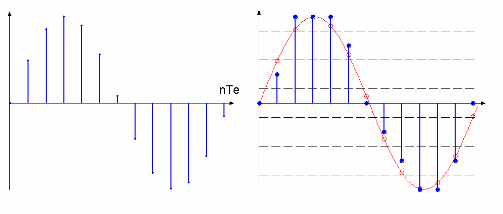
\includegraphics[scale=0.6]{CAN.png}
\caption{Discrétisation et échantillonnage}
\end{figure}

La limitation d'amplitude est source de saturation du signal échantillonné. La quantification génère un bruit sur le signal en sortie du CAN (appelé bruit de quantification). Ce bruit peut être modélisé par une variable aléatoire  de moyenne nulle, de répartition uniforme et de variance donnée par $q^2 / 12 $.\\

Dans le cadre de ce cours, on fera l'hypothèse que la quantification ne génère pas de bruit de quantification. Il n'y auras pas non plus de saturation : on parle de numérisation parfaite.\\

Remarque : ces opérations induisent également des retards de l'information. \\

Conséquence : en amont du CAN, on place un FAR\footnote{Filte anti-repliement de spectre} , un filtre analogique passe-bas.

\subsection*{Convertisseur Numérique Analogique}

Problématique : transformer un échantillon numérique en signal analogique défini $\forall t$.

Challenge théorique : quel comportement entre $(k-1)T_e$ et $kT_e$.

Idée : extrapolation des échantillons entre 2 instants d'échantillonnage.

\paragraph{Cas du Bloqueur d'Ordre Zéro}

$B_0(p)$ fonction de transfert du filtre réalisant le BOZ.
\[b_0(t) = 1_0^+(t) - 1_0^+(t-T_e)\]
Donc par transformée de Laplace inverse,
\[B_0(p) = \frac{1}{p}-\frac{1}{p}e^{-T_ep} \]
\[ \boxed{B_0(p) = \frac{1-e^{-T_ep}}{p}} \]


\end{document}
